\documentclass{beamer}
\usepackage{graphicx, epstopdf}
\usepackage{grffile}
\usepackage{amsmath, amssymb, amsbsy, amstext}
% \usepackage{xcolor}

\usepackage[utf8]{inputenc}
\usepackage{natbib}

\usepackage{todonotes}
% \usepackage[disable]{todonotes}
\presetkeys{todonotes}{inline}{}

\usepackage{booktabs} % for much better looking tables
\usepackage{tabularx}

\newcommand{\code}[1]{{\texttt{#1}}}
\newcommand{\libraryname}[1]{{\texttt{#1}}}
\newcommand{\codefile}[1]{{\textit{#1}}}
\newcommand{\program}[1]{\code{#1}}
\newcommand{\taskname}[1]{{\textit{#1}}}
\newcommand{\newterm}[1]{{\textit{#1}}}
\newcommand{\scarequotes}[1]{`#1'}
\newcommand{\sampleswidth}{0.23\textwidth}
\newcommand{\samplesheight}{1.5cm}

% \definecolor{darkgreen}{rgb}{0,0.6,0}
% \usepackage{pgf}
% \logo{\pgfputat{\pgfxy(-2,6)}{\pgfbox[center,base]{\includegraphics[height=2cm]{amsilogo.jpg}}}}

\usetheme{Darmstadt} 
%\usetheme{Dresden} %Dresden, Darmstadt, Warsaw
% \usecolortheme{dove}
% \title{Sphere Detection using Boosted Classifiers}
\title{Comparing Feature Desctiptor Performance of Boosted Classifiers }
% \subtitle{Computer Vision Interim Report}
\author{Brendan Annable, Mitchell Metcalfe, Monica Olejniczak}
\institute{The University of Newcastle, Australia}
\date{\today}

\begin{document}

	\maketitle

	
	% \begin{frame}{Object detection}
	% 	\begin{center}
	% 		To create an object detector using supervised learning, a correctly
	% 		labelled dataset needs to be created for training.
	% 	\end{center}
	% \end{frame}

\section{Introduction}

	\subsection{Motivation}

	\begin{frame}{Robot soccer}
		Robots at RoboCup \citep{KitanoAKNO97} need to know where the ball is. Basic approach is circle detection, which has problems: \par
		\begin{itemize}
			\item Centre circle
	        \item Penalty spots
	        \item Line intersections
	        \item Anything that looks round from some angle
		\end{itemize}
	\end{frame}

	\begin{frame}{Current approaches}
		A review of recent literature reveals several recent approaches:
		\todo{Something}
	\end{frame}

	\begin{frame}{Sphere detection problem}
		\begin{itemize}
			\item More general problem than ball detction.
			\item Detect spheres.
			\item Do not detect any \scarequotes{round things} unless they are spheres.
		\end{itemize}
		\begin{table}[h]
			\centering
			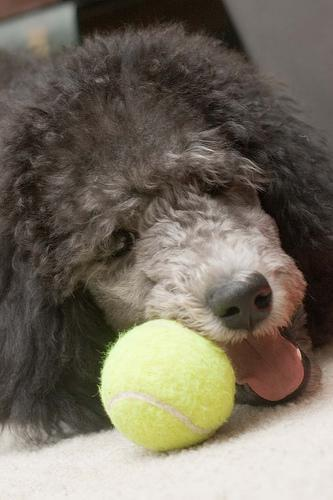
\includegraphics[height=4cm]{training_images/positive/n04409515_2793} \hspace*{0.1cm}
			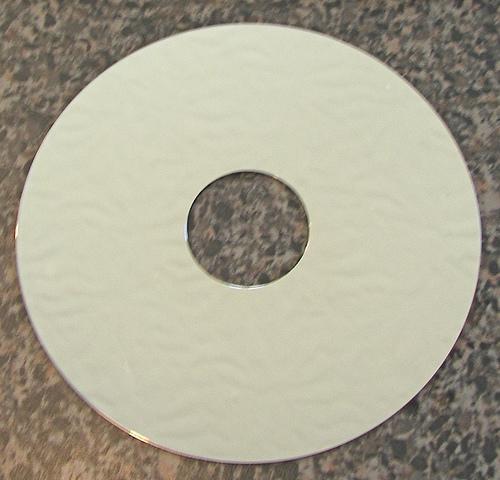
\includegraphics[height=4cm]{training_images/hard_negative/n03208556_9694}
		\end{table}
	\end{frame}

\section{Focus of work}
	\begin{frame}{Proposed approach}
		Attempt to solve the more generic problem of sphere detection using a boosted classifier cascade.
	\end{frame}

	\begin{frame}{Feature comparison}
		Compare appropriateness of the following feature types for the problem: \par
		\begin{itemize}
			\item Extended Haar features \citep{Lienhart2002extended}
			\item Local Binary Patterns (LBPs) \citep{liao2007learning}
			\item Histograms of Oriented Gradients (HoG) features \citep{dalal2005histograms}
		\end{itemize}
	\end{frame}

\section{Methodology}
	% 
	%  (describe the goal of comparing techniques)

\section{Training}

\begin{frame}{Dataset}
	All training and testing images were sourced from ImageNet \citep{imagenet_cvpr09}.
\end{frame}

\begin{frame}{Positive samples}
	\begin{table}[H]
		\footnotesize
		\centering
		\caption{ImageNet synsets used for the positive samples in the training set and their associated WordNet \citep{fellbaum1998wordnet} identifiers.}
		\label{tab:postraining}
		\begin{tabularx}{\textwidth}{lX}
			\toprule
			\textbf{Id} & \textbf{Category} \\
			\midrule
			n02799071 & Baseball \\
			n02802426 & Basketball \\
			n02882301 & Bowling ball, bowl \\
			n03134739 & Croquet ball \\
			n03145719 & Cue ball \\
			n03267113 & Eight ball \\
			n03721047 & Marble \\
			n03742019 & Medicine ball \\
			n03825442 & Ninepin ball, skittle ball \\
			n03942813 & Ping-pong ball \\
			n03982232 & Pool ball \\
			n04409515 & Tennis ball \\
			n04540053 & Volleyball \\
			\bottomrule
		\end{tabularx}
	\end{table}
\end{frame}

\begin{frame}{Positive samples (\scarequotes{Simple})}
	\begin{table}[H]
		\footnotesize
		\centering
		\caption{ImageNet synsets used for the positive samples in the training set and their associated WordNet \citep{fellbaum1998wordnet} identifiers.}
		\label{tab:postraining}
		\begin{tabularx}{\textwidth}{lX}
			\toprule
			\textbf{Id} & \textbf{Category} \\
			\midrule
			\textcolor{red}{n02799071} & \textcolor{red}{Baseball} \\
			n02802426 & Basketball \\
			n02882301 & Bowling ball, bowl \\
			\textcolor{red}{n03134739} & \textcolor{red}{Croquet ball} \\
			\textcolor{red}{n03145719} & \textcolor{red}{Cue ball} \\
			n03267113 & Eight ball \\
			n03721047 & Marble \\
			n03742019 & Medicine ball \\
			\textcolor{red}{n03825442} & \textcolor{red}{Ninepin ball, skittle ball} \\
			\textcolor{red}{n03942813} & \textcolor{red}{Ping-pong ball} \\
			\textcolor{red}{n03982232} & \textcolor{red}{Pool ball} \\
			n04409515 & Tennis ball \\
			n04540053 & Volleyball \\
			\bottomrule
		\end{tabularx}
	\end{table}
\end{frame}

\begin{frame}{Test set}
	\begin{table}[H]
		\centering
		\caption{Additional WordNet identifiers for positive samples in the test set.}
		\label{tab:postest}
		\begin{tabularx}{\textwidth}{lX}
			\toprule
			\textbf{Id} & \textbf{Category} \\
			\midrule
				n02778669 & Ball \\
				n02779435 & Ball \\
				n02839351 & Billiard ball \\
				n02778669 & Generic sporting equipment balls \\
				n03445777 & Golf ball \\
				n02779435 & Plaything, toy, ball \\
				n04254680 & Soccer ball \\
			\bottomrule
		\end{tabularx}
	\end{table}
\end{frame}

\begin{frame}{Negative samples}
	\begin{table}[H]
		\centering
		\caption{WordNet identifiers for hard negative samples in the training set.}
		\label{tab:negtraining}
		\begin{tabularx}{\textwidth}{lX}
			\toprule
			\textbf{Id} & \textbf{Category} \\
			\midrule
				n03032811 & Circle, round \\
				n13873917 & Circle \\
				n13873502 & Circle \\
			\bottomrule
		\end{tabularx}
	\end{table}
\end{frame}

\begin{frame}{Background samples}
	\begin{table}[H]
		\centering
		\caption{WordNet identifiers for background samples in the test set.}
		\label{tab:baktraining}
		\begin{tabularx}{\textwidth}{lX}
			\toprule
			\textbf{Id} & \textbf{Category} \\
			\midrule
				n02782778 & Ballpark, park \\
				n08659446 & Field \\
				n03841666 & Office, business office \\
			\bottomrule
		\end{tabularx}
	\end{table}
\end{frame}

\begin{frame}{Samples}
	\begin{table}[H]
		\centering
		\tabcolsep=0.11cm
		\begin{tabularx}{\textwidth}{@{}XXXX@{}}
			% Positive
			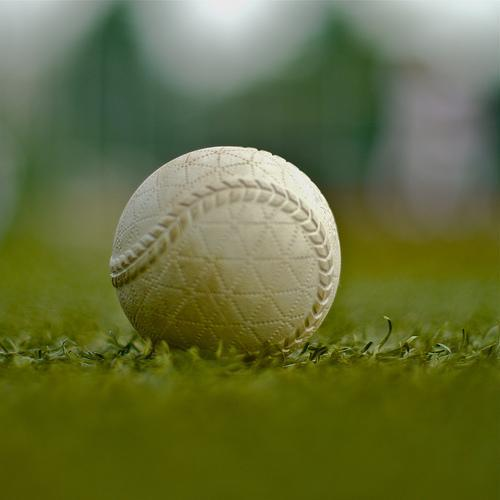
\includegraphics[height=\samplesheight]{training_images/positive/n02799071_17616} &
			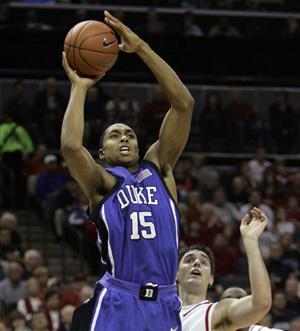
\includegraphics[height=\samplesheight]{training_images/positive/n02802426_6256} &
			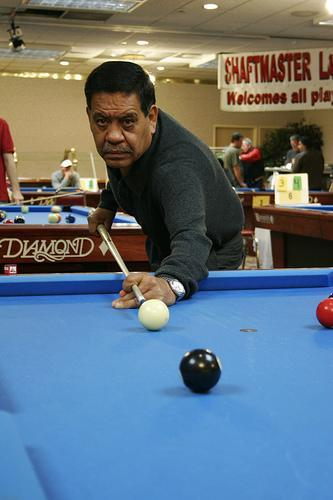
\includegraphics[height=\samplesheight]{training_images/positive/n03145719_8658} &
			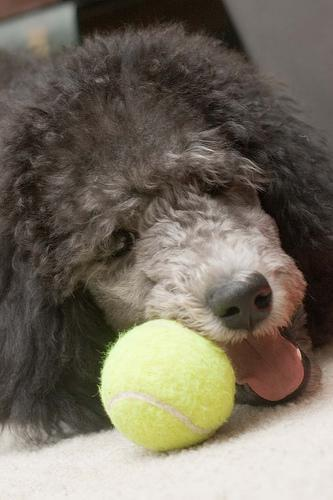
\includegraphics[height=\samplesheight]{training_images/positive/n04409515_2793} \\
			% Positive thumbnails
			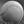
\includegraphics[height=\samplesheight]{training_images/positive/n02799071_17616.thumbnail.jpg} &
			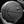
\includegraphics[height=\samplesheight]{training_images/positive/n02802426_6256.thumbnail.jpg} &
			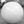
\includegraphics[height=\samplesheight]{training_images/positive/n03145719_8658.thumbnail.jpg} &
			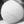
\includegraphics[height=\samplesheight]{training_images/positive/n04409515_2793.thumbnail.jpg} \\
			% Hard negative
			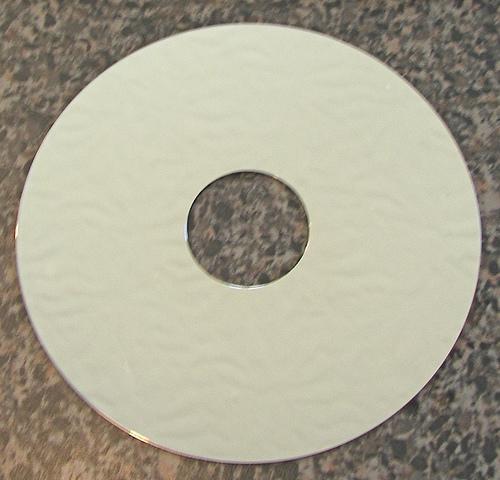
\includegraphics[height=\samplesheight]{training_images/hard_negative/n03208556_9694} &
			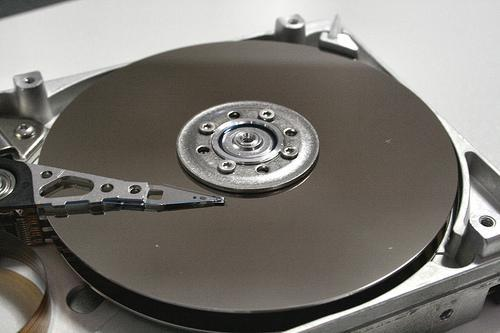
\includegraphics[height=\samplesheight]{training_images/hard_negative/n03208556_11973} &
			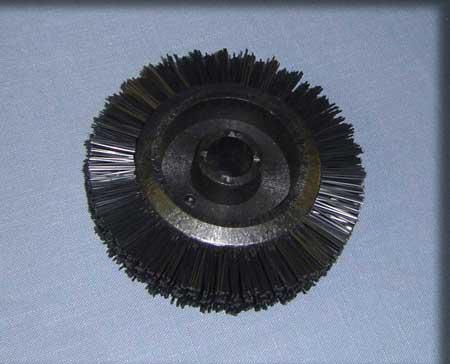
\includegraphics[height=\samplesheight]{training_images/hard_negative/n03208556_13484} &
			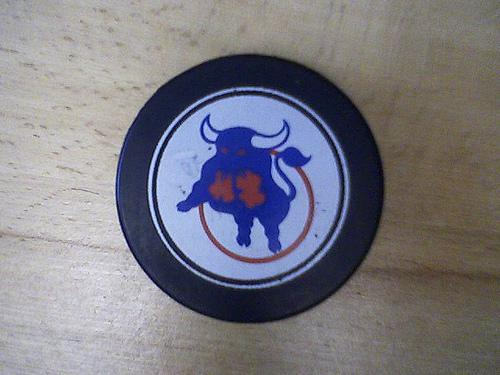
\includegraphics[height=\samplesheight]{training_images/hard_negative/n04019541_26831} \\
			% Hard negative thumbnails
			
\includegraphics[height=\samplesheight]{training_images/hard_negative/n03208556_9694.thumbnail.jpg} &
			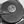
\includegraphics[height=\samplesheight]{training_images/hard_negative/n03208556_11973.thumbnail.jpg} &
			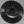
\includegraphics[height=\samplesheight]{training_images/hard_negative/n03208556_13484.thumbnail.jpg} &
			
\includegraphics[height=\samplesheight]{training_images/hard_negative/n04019541_26831.thumbnail.jpg}
		\end{tabularx}
	\end{table}
\end{frame}

\begin{frame}{Software used}
	\begin{itemize}
		\item Classifiers of each feature type were trained simultaneously
		\item Run on a Macbook Pro with an Intel Core i7 (I7-3740QM) processor and 16GB RAM.
	\end{itemize}
\end{frame}


\section{Results}

% Make a table of results
% Hopefully a graph?

\begin{frame}{Training results}
	\begin{table}[H]
		\footnotesize
		\centering
		% \caption{Results for all training schemes}
		% \label{tab:trainresults}
		\begin{tabularx}{\textwidth}{lcccccc}
			\toprule
			\textbf{name} & \textbf{number} & \textbf{posFrag} & \textbf{hardNegFrac} & \textbf{fullset} & \textbf{type} & \textbf{hitrate} \\
			\midrule
			\(scheme_1\) & 2000 & 0.33 & 0 & 0 & HAAR & 9.09\% \\
			\(scheme_2\) & 2000 & 0.33 & 0.25 & 0 & HAAR & 6.49\% \\
			\(scheme_3\) & 2000 & 0.33 & 0.25 & 0 & HAAR & 16.45\% \\
			\(scheme_4\) & 4000 & 0.5 & 0.2 & 1 & HAAR & 19.91\% \\
			\(scheme_5\) & 3500 & 0.5 & 0 & 1 & HAAR & 20.35\% \\
			\(lbp_1\) & 2000 & 0.33 & 0 & 0 & LBP & 01.73\% \\
			\(lbp_2\) & 2000 & 0.33 & 0.25 & 0 & LBP & 3.03\% \\
			\(lbp_3\) & 2000 & 0.33 & 0.25 & 0 & LBP & 4.76\% \\
			\(lbp_4\) & 4000 & 0.5 & 0.2 & 1 & LBP & 6.06\% \\
			\(lbp_5\) & 3500 & 0.5 & 0 & 1 & LBP & 8.23\% \\
			\(hog_1\) & 2000 & 0.33 & 0 & 0 & HOG & 1.3\% \\
			\(hog_2\) & 2000 & 0.33 & 0.25 & 0 & HOG & 0.87\% \\
			\(hog_3\) & 2000 & 0.33 & 0.25 & 0 & HOG & 2.6\% \\
			\(hog_4\) & 4000 & 0.5 & 0.2 & 1 & HOG & 3.03\% \\
			\(hog_5\) & 3500 & 0.5 & 0 & 1 & HOG & 5.19\% \\
			\bottomrule
		\end{tabularx}
	\end{table}
\end{frame}

\begin{frame}{Trial comparison chart}
	\begin{center}
		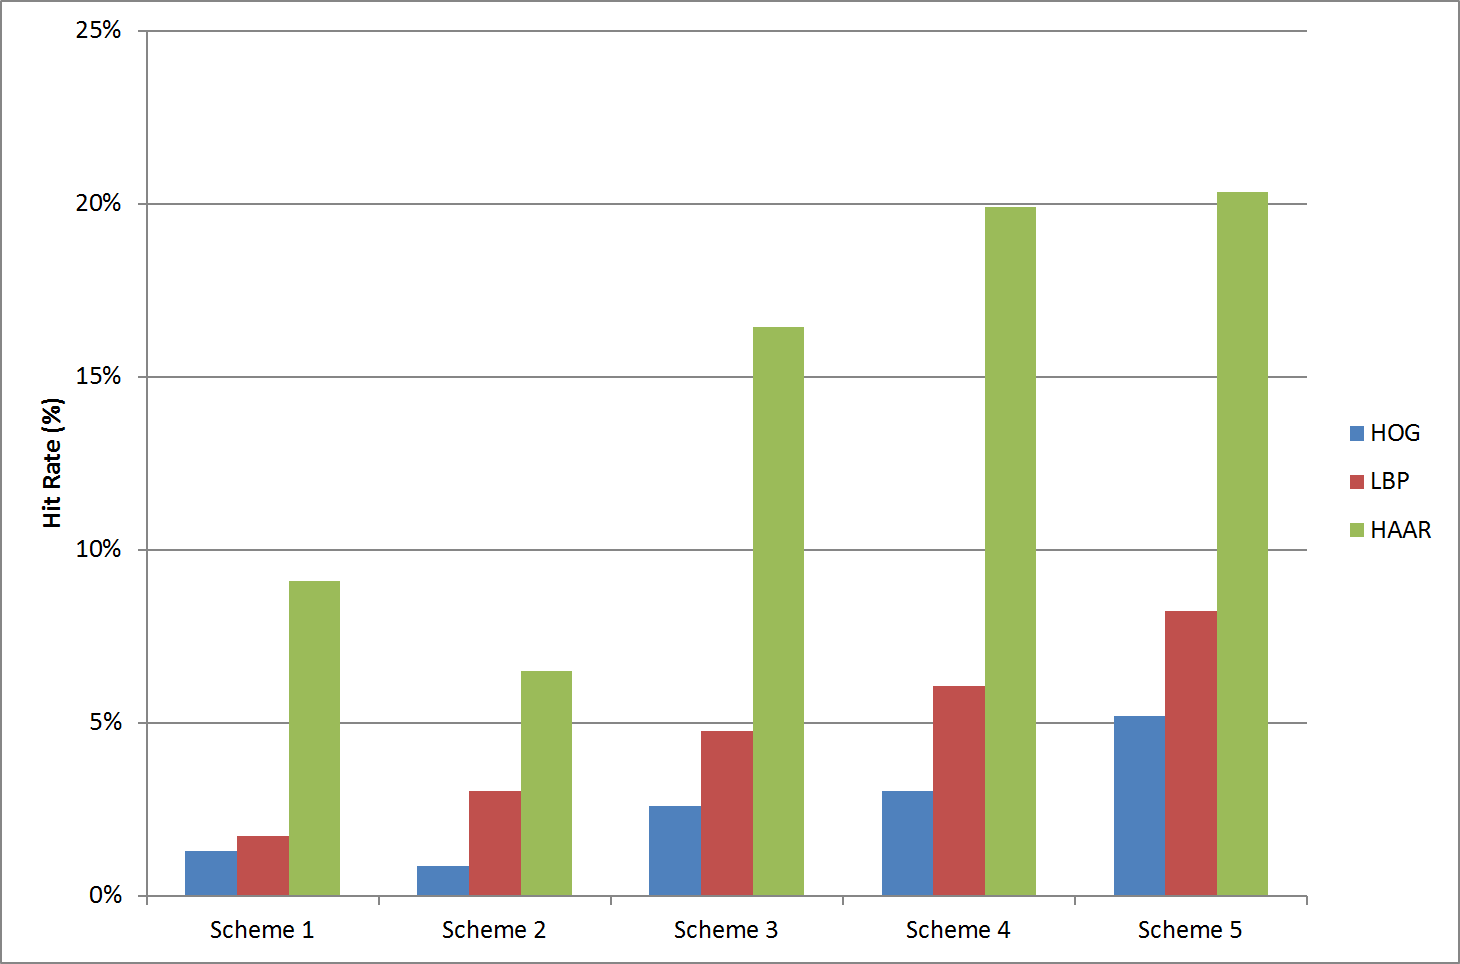
\includegraphics[width=0.9\textwidth]{results_graph}
	\end{center}
\end{frame}

\section{Conclusion}

	\subsection{Feature performance comparison}
	%   - Haar features clearly performed better than HOGS or LBP on the sphere detection task
	%   - 

	\subsection{Future work}
	% Future Work
	%   - 

	\subsection{Bibliography}

	\begin{frame}{Bibliography}
		\bibliography{references}
		\bibliographystyle{apalike}
	\end{frame}

\end{document}

